\documentclass[paper=a4, parskip=half-, ngerman, fontsize=11pt]{scrreprt}
\usepackage[T1]{fontenc}

\usepackage[ngerman]{babel}
\babelprovide[hyphenrules=ngerman-x-latest]{ngerman}

\usepackage{csquotes}
\usepackage[backend=biber]{biblatex}
\addbibresource{Proseminar.bib}

\usepackage{graphicx}
\usepackage{url}


\begin{document}

% Titelseite
\begin{titlepage}
    \begin{center}
        % Unilogo oben
        
\includegraphics[width=0.5\textwidth]{logo_fernuni_hagen.png}\\[2cm]

        {\LARGE \textbf{Übertragung von Signalen auf elektrischen Leitungen}}\\[2cm]

        \textbf{Proseminar Mathematik in der Technik}\\
        \textbf{Modulnummer:} 61711\\
        Fakultät für Mathematik + Informatik\\[0.5cm]

        \begin{tabbing}
            \hspace{6cm} \= \kill
            \textbf{Name:} \> Sven Schmidt \\
            \textbf{Matrikelnummer:} \> 4125169 \\
            \textbf{Abgabedatum:} \> \today \\
            \textbf{Prüfer:} \> PD Dr.-Ing. Stefan Helfert \\
        \end{tabbing}

        \vfill

        {\large FernUniversität in Hagen}\\
        {\large Sommersemester 2025}
    \end{center}
\end{titlepage}

\chapter{Einführung}

\chapter{Modell des Zweidrahtleiters}

In dieser Ausarbeitung beschränken wir uns auf die Untersuchung der Ausbreitung elektromagnetischer Wellen in
Zweidrahtleitern (Paralleldraht), die schematisch in der folgenden Abbildung gezeigt.
\begin{figure}[!h]
    \begin{center}
        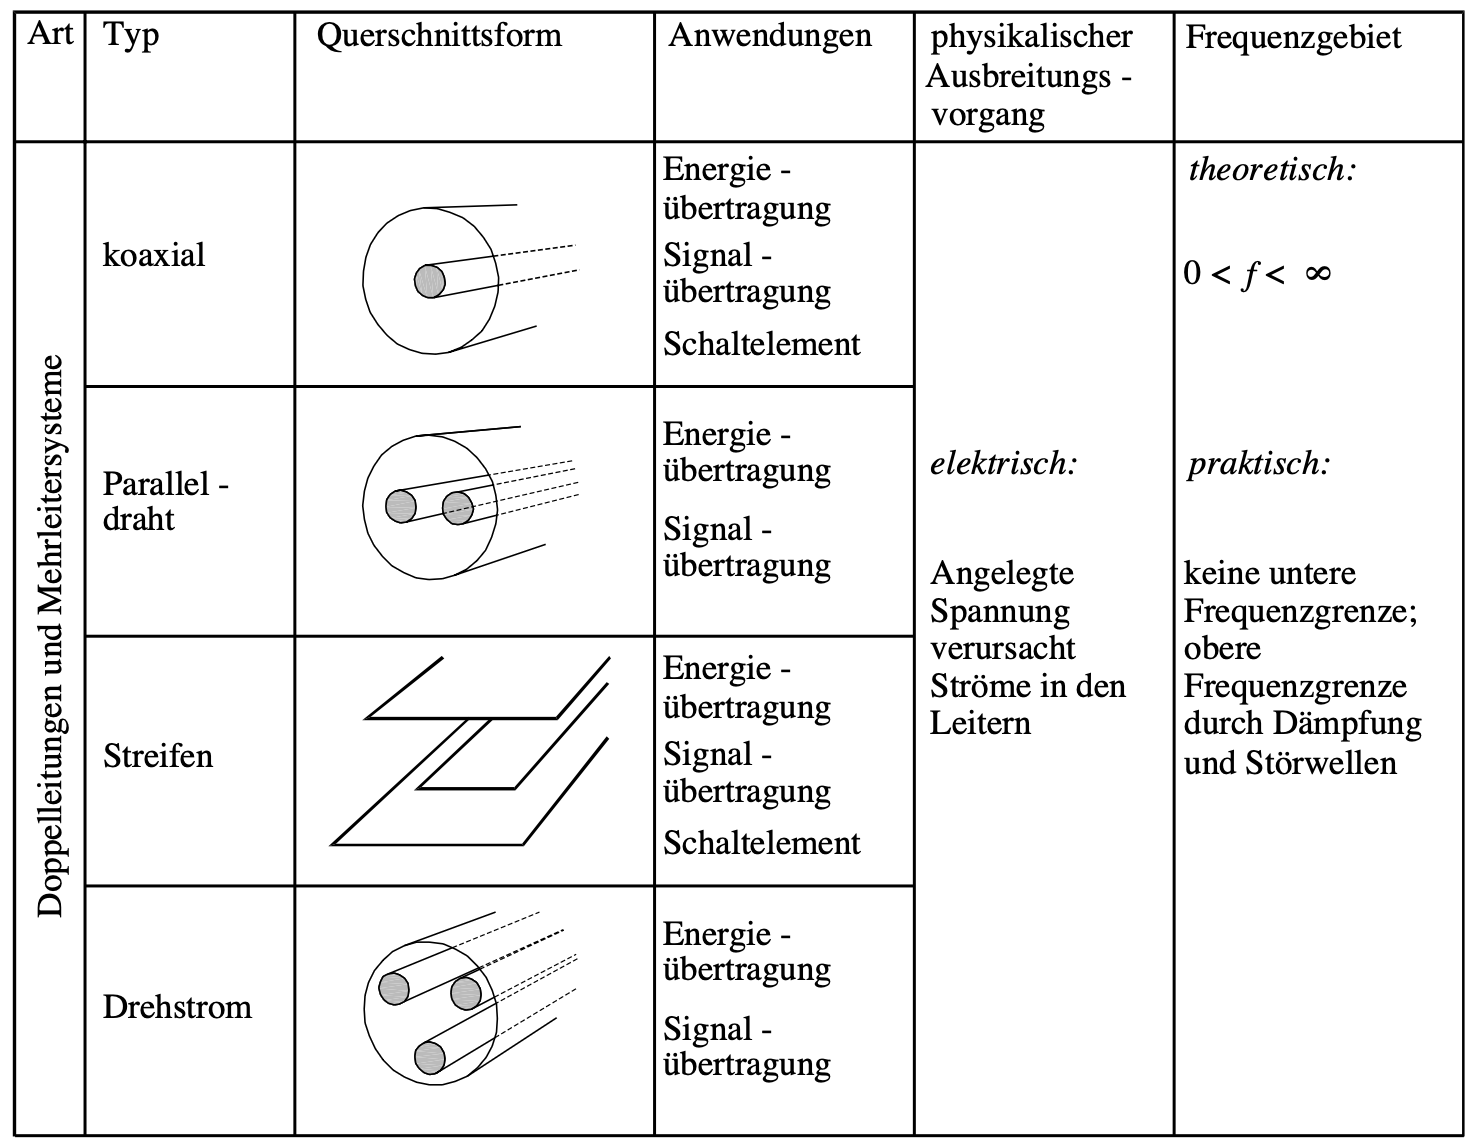
\includegraphics[width=0.5\textwidth]{images/Leiter.png}
        \caption{Elektrische Leiter mit ihren Anwendungen. Entnommen aus~\cite{FernuniSkript}.}
        \label{Leiter}
    \end{center}
\end{figure}

Aus den Gesetzen der Elektro- und Magnetostatik ist bekannt, dass sich beim Durchfließen eines elektrischen Stroms um
den Leiter ein magnetisches Feld ausbildet. Analog bildet die Potenzialdifferenz beider Leiter ein elektrisches Feld
aus. Die folgende Abbildung~\ref{Felder} zeigt den Querschnitt eines Leiters mit eingezeichneten Feldlinien.

\begin{figure}[!h]
    \begin{center}
        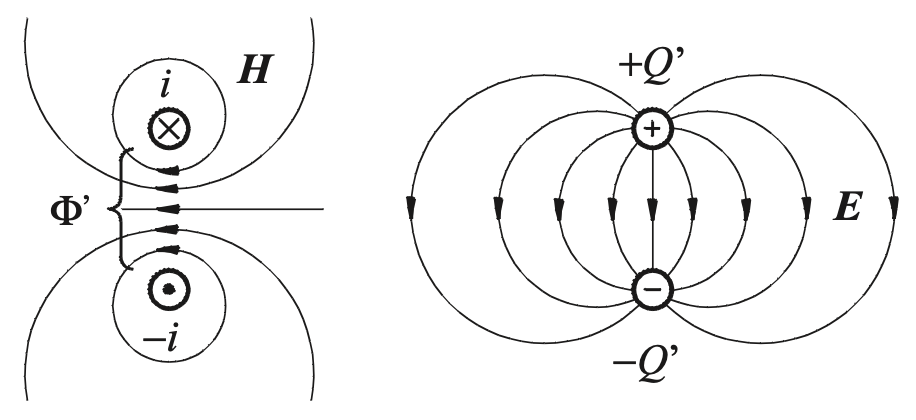
\includegraphics[width=0.5\textwidth]{images/Felder.png}
        \caption{Elektrische Leiter mit ihren Anwendungen. Entnommen aus~\cite{LeitungenUndFilter}.}
        \label{Felder}
    \end{center}
\end{figure}

Im Folgenden nehmen wir an, dass der Abstand $d$ zwischen den Leitern viel kleiner ist, als die Wellenlänge $\lambda$
der auftretenden Signale,
\[ d \ll \lambda = \frac{c_{0}}{f \sqrt{\epsilon_{r}}} \]
wobei $c_{0}$ die Lichtgeschwindigkeit im Vakuum, $f$ die Frequenz des Signals und $\epsilon_{r}$ die relative
Dielektrizitätskonstante bezeichnet. Wir machen hier die vereinfachende Annahme, dass $\epsilon_{r}$ eine (konstante)
Eigenschaft des Mediums ist, in dem sich das Signal ausbreitet. Im Vakuum gilt $\epsilon_{r} = 1$.

Wir betrachten nun ein kleines, infinitesimales Leitungsstück $ds$,
\begin{figure}[!h]
    \begin{center}
        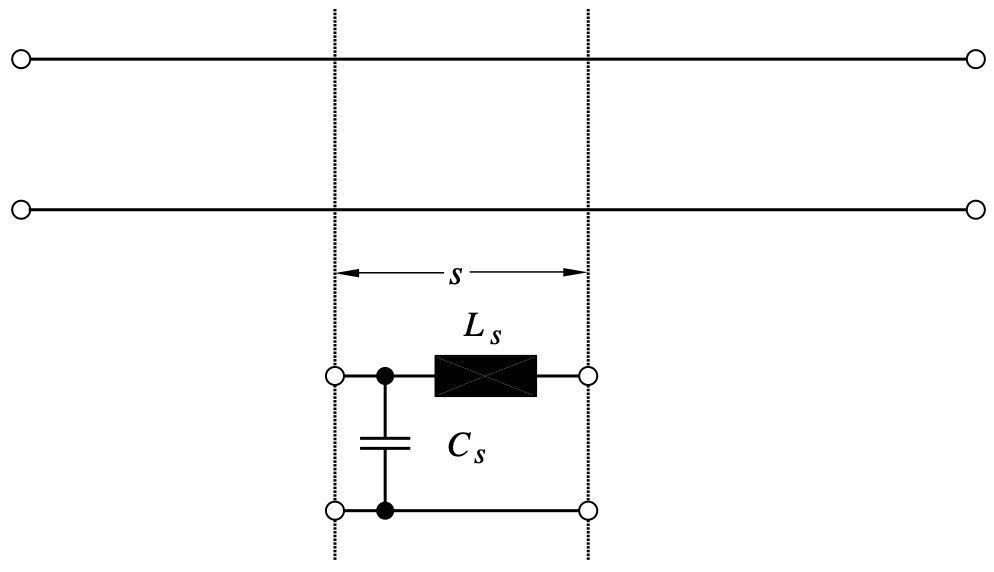
\includegraphics[width=0.5\textwidth]{images/Leitung1.png}
        \caption{Elektrische Leiter mit ihren Anwendungen. Entnommen aus~\cite{LeitungenUndFilter}.}
        \label{Leitung1}
    \end{center}
\end{figure}

Der Fluss $\Phi$ des magnetischen Feldes $\textbf{H}$ bewirkt eine Induktivität $L_{s}$
\[ \Phi_{s} = i \cdot L_{s} \], wobei $i$ der Strom ist.
Das elektrische Feld $\textbf{E}$ induziert Ladungen auf der Oberfläche des Leiters und damit eine Kapazität $C_{s}$,
die über die Spannung $u$ wie folgt zusammenhängt,
\[ Q_{s} = C_{s} \cdot u . \]
Die gesamte Leitung stellen wir uns aus diesen Leitungsstücken zusammengesetzt vor wie auf Abbildung~\ref{Leitung2}
dargestellt.
\begin{figure}[!h]
    \begin{center}
        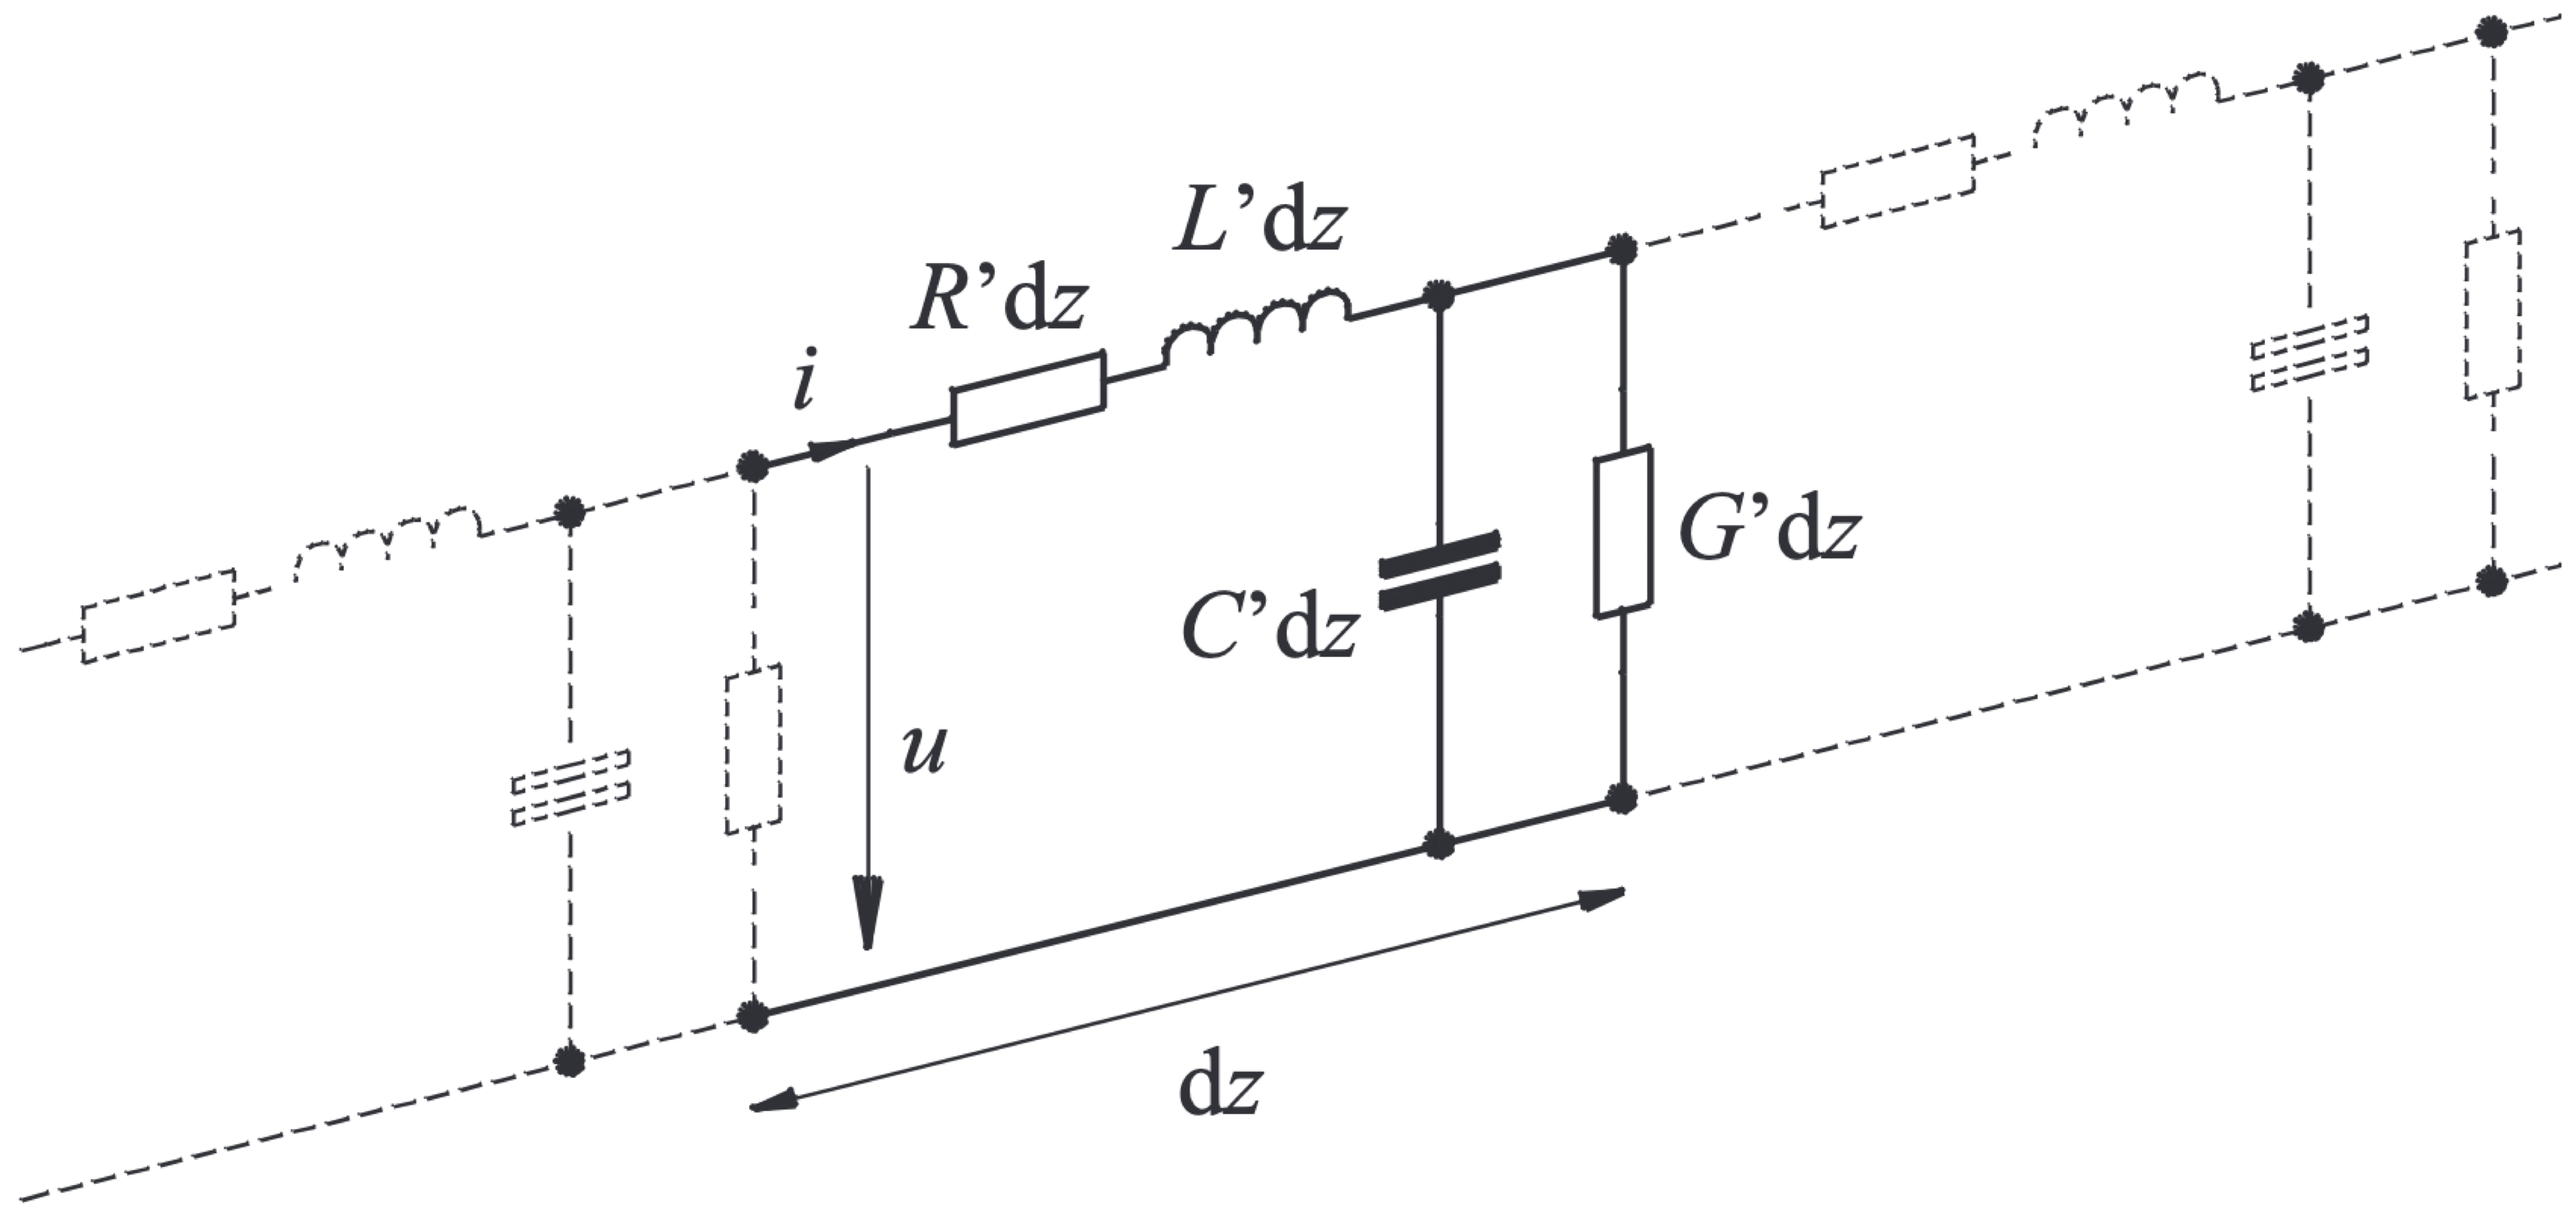
\includegraphics[width=0.5\textwidth]{images/Leitung2.png}
        \caption{Elektrische Leiter mit ihren Anwendungen. Entnommen aus~\cite{LeitungenUndFilter}.}
        \label{Leitung2}
    \end{center}
\end{figure}
Die führt auf die folgenden qualitativen Eigenschaften: Wir eine Spannung am Leitungsanfang angelegt, muss zunächst die
erste Kapazität $Q_{s_{1}}$ aufgeladen werden. Erst dann bildet sich eine Spannung an der Längsinduktivität $L_{s_{1}}$
an. Der aufgebaute Strom wird nun $Q{s_{2}}$ aufladen etc., bis zum Leiterende. Die Ausbreitung des Einschaltvorgangs
findet mit endlicher Geschwindigkeit statt.





\chapter{Telegraphenleitungen}

\section{Verlustloses Model}

\section{Verlustbehaftetest Model}

\section{Abschlüsse}


%\bibliographystyle{plain} % oder ein anderer Stil, z.B. alpha, abbrv, unsrt
%\bibliography{Proseminar} % Name Ihrer .bib-Datei OHNE Endung .bib
\printbibliography

\end{document}